\documentclass[12pt]{article}
\usepackage{times} 			% use Times New Roman font

\usepackage[margin=1in]{geometry}   % sets 1 inch margins on all sides
\usepackage{hyperref}               % for URL formatting
\usepackage[pdftex]{graphicx}       % So includegraphics will work
\setlength{\parskip}{1em}           % skip 1em between paragraphs
\usepackage{indentfirst}            % indent the first line of each paragraph
\usepackage{datetime}
\usepackage[small, bf]{caption}
\usepackage{listings}               % for code listings
\usepackage{xcolor}                 % for styling code
\usepackage{multirow}
\usepackage{float}
\usepackage{csvsimple}
\usepackage{ragged2e}
\usepackage{cite}

%New colors defined below
\definecolor{backcolour}{RGB}{246, 246, 246}   % 0xF6, 0xF6, 0xF6
\definecolor{codegreen}{RGB}{16, 124, 2}       % 0x10, 0x7C, 0x02
\definecolor{codepurple}{RGB}{170, 0, 217}     % 0xAA, 0x00, 0xD9
\definecolor{codered}{RGB}{154, 0, 18}         % 0x9A, 0x00, 0x12

%Code listing style named "gcolabstyle" - matches Google Colab
\lstdefinestyle{gcolabstyle}{
  basicstyle=\ttfamily\small,
  backgroundcolor=\color{backcolour},   
  commentstyle=\itshape\color{codegreen},
  keywordstyle=\color{codepurple},
  stringstyle=\color{codered},
  numberstyle=\ttfamily\footnotesize\color{darkgray}, 
  breakatwhitespace=false,         
  breaklines=true,                 
  captionpos=b,                    
  keepspaces=true,                 
  numbers=left,                    
  numbersep=5pt,                  
  showspaces=false,                
  showstringspaces=false,
  showtabs=false,                  
  tabsize=2
}

\lstset{style=gcolabstyle}      %set gcolabstyle code listing

% for fancy page headings
\usepackage{fancyhdr}
\setlength{\headheight}{13.6pt} % to remove fancyhdr warning
\pagestyle{fancy}
\fancyhf{}
\rhead{\small \thepage}
\lhead{\small Documentation}  % EDIT THIS
\chead{\small JetPack Compose and RoomDatabase Design Practices} 

%-------------------------------------------------------------------------
\begin{document}

\begin{centering}
{\large\textbf{Android Template Code}}\\ % EDIT THIS
                                % REPLACE # with HW num and ADD title
Jacob Conner\\                     % EDIT THIS
September 27, 2021\\                      % EDIT THIS
\end{centering}

%-------------------------------------------------------------------------
\tableofcontents

% The * after \section just says to not number the sections
\section{Gradle}
This section examines the \textit{build.gradle} files in the Project and App folders and the project \textit{Build.settings} files. 
\newpage
\subsection{ProjectBuildGradle}
\lstinputlisting[language=Java, caption=Project build.gradle file, label={lst:projectBuildGradle}]{build.gradle}
All Android projects consist of at least two \textit{build.gradle} files, a project level \textit{build.gradle} file and an application level \textit{build.gradle} file. The project level \textit{build.gradle} file is shown in Listing  \ref{lst:projectBuildGradle}. Generally this 
\textit{build.gradle} file contains a \verb|buildscript| tag that has a number of subsections. The section mostly likely to be 
editted is the \verb|ext| section. In this section gradle environment variables can be defined particularly to keep track 
of versions of various dependencies. In this example the \verb|compose_version| variable is defined with \verb|compose_version = '1.0.1'|. Dependencies can be defined in this section but generally should be defined using the application level \textit{build.gradle} file. 

\newpage

\subsection{AppBuildGradle}
\lstinputlisting[language=Java, caption=App build.gradle file, label={lst:appBuildGradle}]{app/build.gradle}
This app-level  \textit{build.gradle} file is used to define the various plugins, application dependencies and gradle scripts pertinent to the application. In the example file in Listing \ref{lst:appBuildGradle} the file starts with plugins section. The plugins section consists of four plugins.:
\begin{itemize}
    \item com.android.application
    \item kotlin-android
    \item Kapt plugin - kotlin-kapt
    \item Dokka plugin - org.jetbrains.dokka
\end{itemize}
\verb|com.android.application| and \verb|kotlin-android| are all included in the application by default. This example has added the plugin \verb|kotlin-kapt| to enable the program to load the room compiler dependency using the kapt command. The dokka plugin needed to create documentation using KDoc is added with the \verb|id("org.jetbrains.dokka") version "1.4.0"|.
Various gradle tasks should be added in the application \textit{build.gradle} file. 
\begin{lstlisting}[numbers=none, 
			caption=Task to generate Dokka documentation,
			label={lst:dokkatask}]
tasks.dokkaHtml.configure {
    outputDirectory.set(file("../documentation/html"))
}
\end{lstlisting}
The task to generate dokka documentation is defined using the code in Listing \ref{lst:dokkatask} . Gradle documentation can be created using the terminal with the command \verb|gradlew dokkaHtml|. Dokka will then parse all KDoc comment lines in Kotlin classes and generate the documentation in the build/dokka folder. 

Dependencies are stored in the dependencies section of the \textit{build.gradle} file. When a new empty compose application is created, a number of compose dependencies are included as well as various testing frameworks. The Jetpack compose navigation library and the jetpack compose lifecycle libraries are not included by default but are present in the example app \textit{build.gradle} file. The project also makes use of RoomDatabase library so those libraries are included. In order to allow for the downloading and display of images from the internet the \verb|io.coil-kt:coil-compose| library is included. 


\newpage
\section{AndroidManifest}
\lstinputlisting[language=xml, caption=Android Manifests File, label={lst:androidXML}]{app/src/main/AndroidManifest.xml}
The \textit{android.manifest} file shown in \ref{lst:androidXML} provides information about the various permissions in the application. 

\begin{lstlisting}[numbers=none, 
			caption=Line to give permission to allow internet access,
			label={lst:internetPermission}]
<uses-permission android:name="android.permission.INTERNET" />
\end{lstlisting}

\begin{lstlisting}[numbers=none, 
			caption=Line to give permission to allow network access,
			label={lst:networkPermission}]
<uses-permission android:name="android.permission.ACCESS_NETWORK_STATE"/>
\end{lstlisting}
The most common reason to edit this file is when an application needs to have access to a website or other resource. Internet access is enabled with the line shown in Listing \ref{lst:internetPermission}.
Network access is also needed to allow the application to access the web, and this is enabled with the line in Listing \ref{lst:networkPermission}.


\newpage

\section{RoomDatabase}
The RoomDatabase library is an object relational mapping (ORM) library in Android that serves as a layer for SQLite queries \cite{GoogleRoomDB} .
\subsection{Dependencies}
The implementations are briefly discussed in Section \ref{lst:appBuildGradle}, but a list of the required implementations in the \textit{build.gradle} file are listed below. 

\begin{itemize}
\item RoomDatabase Libraries \begin{itemize}
    \item implementation "androidx.room:room-runtime:\$room\_version"
    \item annotationProcessor "androidx.room:room-compiler:\$room\_version"
    \item implementation "androidx.room:room-ktx:2.3.0"
    \item kapt "androidx.room:room-compiler:2.3.0"
    \end{itemize}
 \item Lifecycle Libraries \begin{itemize}
    \item implementation "androidx.compose.runtime:runtime-livedata:\$compose\_version"
    \item implementation "androidx.lifecycle:lifecycle-livedata-ktx:2.3.1"
    \end{itemize}
\end{itemize}
 \newpage
 
 The model view view model approach taken in this document is largely derived from the Make it Easy tutorial \cite{MakeItEasyRoom1} \cite{MakeItEasyRoom2} \cite{RoomCodeLab}.
 \subsection{Entities}
The lowest level of RoomDatabase is the entity or data model. An entity is simply a data class that describes the schema for a time using Room annotations. The contents of each entity should correspond to the columns of a single SQLite table. 
\lstinputlisting[language=Java, caption=Example entity class, label={lst:exampleEntity}]{app/src/main/java/com/example/roomandapi/entity/TeamMember.kt}

In Listing \ref{lst:exampleEntity}, an example entity class \verb|TeamMember| is provided for a table called team that stores information about members of a team. In this class, the first Room notation encountered is the \verb|@Entity|notation. This notation is called before the data class is defined and is used to help the Room library identify where this model's data will reside in the SQLite database. In this case the table is called \verb|Team| but the data class is called \verb|TeamMember|. 
Next the data class is created using the \verb|data class <nameOfClass>( <contents>)|. It is important to note that a data class in Kotlin does not contain any methods and is simply defined with the parameters using the parentheses that initialize it. 

The next annotation used in this example class is \verb|@PrimaryKey|. This annotation is used to define the column below as a primary key for the table, which means it has to be unique and cannot be null. The notation also has the possible parameter of \verb|(autoGenerate = true)| which advises SQLite to autoincrement that column. 
The last annotation in the example entity class is \verb|@ColumnInfo| which is used to define the name of the table column using the parameter \verb|name="<nameOfColumn>"|. Once the column name has been defined, a variable in kotlin is created for the model which is tied to the table column set. This process is repeated for all columns needed in the table and each column is separated by commas (","). 
 
\subsection{DAO}
Once an entity has been created, a data abstraction object (DAO) has to be created. This is an interface for the entity that maps SQL queries to various methods that can be called. 
\lstinputlisting[language=Java, caption=Example DAO, label={lst:exampleDAO}]{app/src/main/java/com/example/roomandapi/dao/TeamMemberDAO.kt}

An example of an DAO interface is shown in Listing \ref{lst:exampleDAO}. In this file, the interface is annotated as a DAO with the \verb|@DAO| annotation. After the interface header is created with \verb|interface <nameOfDAO>| the various SQL methods are defined with an annotation followed by a method. The first type of SQL Query annotation is \verb|@Query\verb. This annotation takes a SQL query as a parameter.  Then immediately below it, a function is defined that will handle that query and return either an entity or a list of some sort. The \verb|@Query\verb supports parameterized sql queries as shown in the \verb|getById function| and the parameter in the query is used as a parameter in the method tied to that query. 
Room provides a few SQL query annotations that do not require you to specifically type out the SQL query. The \verb|@Insert| annotation takes a list of entities and inserts them into a database using the method below. The option parameter \verb|onConflict = OnConflictStrategy.REPLACE| allows you to specify the conflict strategy with foreign key constraints when a value is inserted.  The \verb|@Update| annotation is used to create an update query where an entity is provided and the values of the entity are used to update the value of the entity in the database. The  annotation  \verb|@Delete|  writes the query to delete the entity in the database that matches the entity provided in the method. 

\subsection{Repository}
\lstinputlisting[language=Java, caption=Example repository class, label={lst:exampleRepo}]{app/src/main/java/com/example/roomandapi/repository/TeamMemberRepository.kt}
In order to simplify the ability to to call the functions in the DAO interface, a repository class is created.An example repository is shown in Listing \ref{lst:exampleRepo}  This repository class takes the DAO interface as an argument. Class methods for each of the DAO functions. In order to support asynchronous methods since a SQL query may not run instantaneously, each method is marked with suspend. Suspend is part of the coroutines library and is used to force a method to run asynchronously on a coroutine. "A coroutine is an instance of suspendable  computation" that is "not bound to any particular thread" that can be suspended and resumed on different threads \cite{kotlinCoroutines}. 

\subsection{Database}
\lstinputlisting[language=Java, caption=Example database class, label={lst:exampleDB}]{app/src/main/java/com/example/roomandapi/database/WCDatabase.kt}

Listing \ref{lst:exampleDB} shows the database class. There should be one database class for each database in the project, but generally one database should suffice for most applications. The database class starts with the \verb|@Database| annotation which abstracts the requirements for any SQLite database using the SQLite connector in a given language. This annotation requires a list of entity classes in the database, a database version, and exportSchema. The database is an abstract class extending the RoomDatabase using the line \verb|abstract class <nameOfDatabase>: RoomDatabase()|. An abstract constructor for each DAO is provided to allow the database to access the sql queries needed by the entity managed by the DAO. The database class has one method, \verb|getInstance| which takes the context of the application. and returns a returns a database object. A database instance is created with the Room.databaseBuilder method and it takes the context of the application provided, the database class and a string with the name of the database. The synchronized method chains fallbackToDestructiveMigration(), which is used for migrations, when they fail and rebuilds the database if the migration fails. The build method is the method that actually builds the database \cite{roomDBMethods}. 

\subsection{Supporting Dates}
\lstinputlisting[language=Java, caption=Converter Class for supporting Dates, label={lst:exampleConverter}]{app/src/main/java/com/example/roomandapi/utility/DateTimeConverter.kt}

SQLite supports 5 data types. 
\begin{itemize}
\item NULL 
\item INTEGER
\item REAL
\item TEXT
\item BLOB
\end{itemize}
A notable omission in the SQLite database is the absence of a Date type. Dates are supported in a variety of ways. They can be stored as an INTEGER as timestamp with the seconds since January 1st, 1970. Another alternative is it can be stored as TEXT variable using ISO8601 strings such as "YYYY-MM-DD". A final option is the Date can be stored as Julian days numbers since November 24th 4714 BC. RoomDatabase does not provide out of the box support for dates likely due to the variety of options to store Dates in SQLite \cite{SqliteDataTypes}. Instead the developer has to create a helper converter class to convert the type of Date variable used in Kotlin to the type used in the SQLite design \cite{RoomDBTypeConverters}. 

In Listing \ref{lst:exampleConverter} an example type converter is provided to convert a date string formatted using the ISO86601 LOCAL\_DATE string. This class contains a formatter which is used to define how the DateTime string is formatted. There are numerous options for date time string formatting supported in Java and Kotlin \cite{DateTimeFormatterDocs}. Once the formatting string has been defined, the converter class contains two methods for converting to and from the LocalDate class. 

\begin{lstlisting}[numbers=none, 
			caption=Task to generate Dokka documentation,
			label={lst:converterAnnotation}]
@TypeConverters(DateTimeConverter::class)
\end{lstlisting}

Once the converter class has been created, it needs to be added to the Database class shown in \ref{lst:exampleDB}.The \verb|@TypeConverters| annotation is used to allow the Database to support those conversions between SQLite types and Kotlin classes. This annotation is added before the database class header and takes the class for the file used as shown in Listing \ref{lst:converterAnnotation} 

\subsection{ViewModel}
\lstinputlisting[language=Java, caption=Example ViewModel class, label={lst:exampleViewModel}]{app/src/main/java/com/example/roomandapi/viewmodel/TeamMemberViewModel.kt}
The view model is the class that GUI will interact with to run queries. This final layer of abstraction 
The view model, class extends the AndroidViewModel class and takes the argument of application as the context. The init function initializes a DAO with the database class's get instance method using application as context and calls the teamMemberDao function to generate the Dao. 

\section{Testing Room}
In Android projects there are two types of unit tests. There are standard Unit Tests that make use of the JUnit library and run like a normal Java or Kotlin project would. The second type of test is the Android  Test which runs a virtualized environment to access the Android Libraries to run the functions that require the Android Framework to run \cite{AndroidTestingFundamentals}. Room Database is one of those examples. 

\subsection{Creating Tests}

\begin{figure}[H]
    \centering
    % trim and clip are used to crop the image, trim=left bottom right top
    % width sets max width, height will be scaled appropriately
    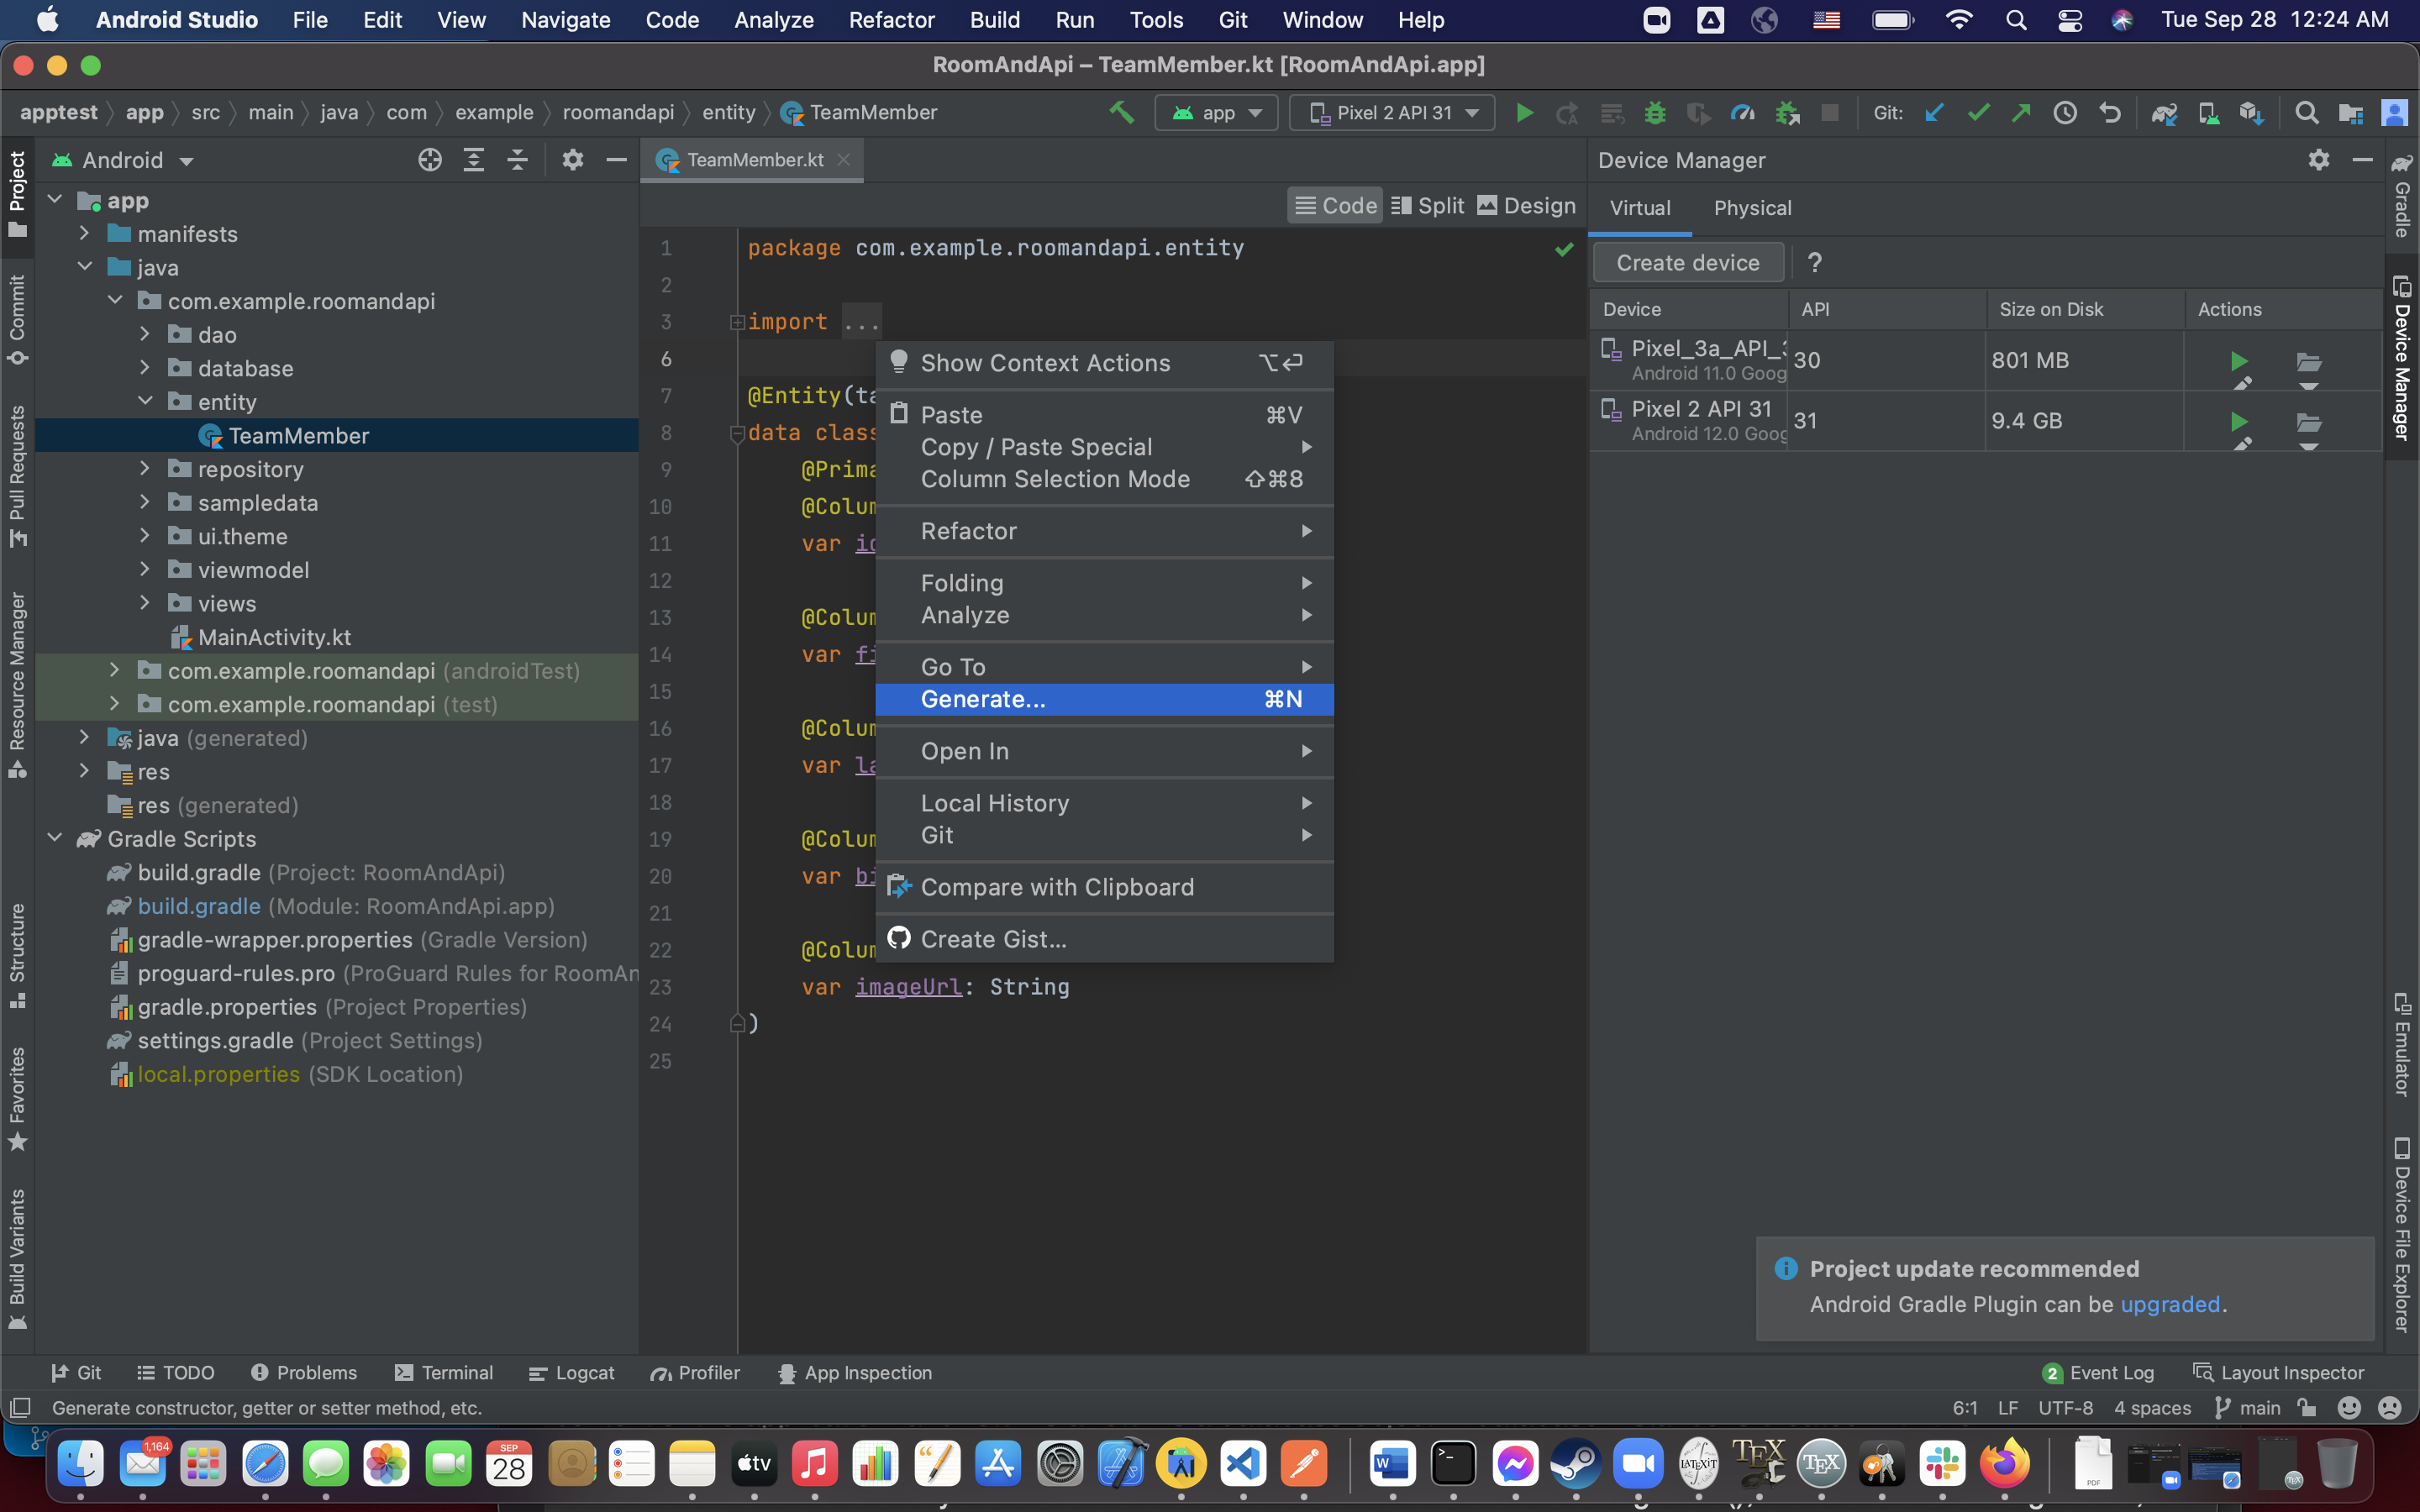
\includegraphics[trim=10 10 10 50, clip, width=\textwidth] {images/testing/1_rightClick.png}
    \caption{Step 1. Open the file you want to test and right click it.}
    \label{fig:test_step_1}
\end{figure}

The process for creating an Android Test with room begins by first navigating to the file that you would like to test. Right click anywhere in the open file and select \verb|Generate...| as shown in Figure \ref{fig:test_step_1}

\begin{figure}[H]
    \centering
    % trim and clip are used to crop the image, trim=left bottom right top
    % width sets max width, height will be scaled appropriately
    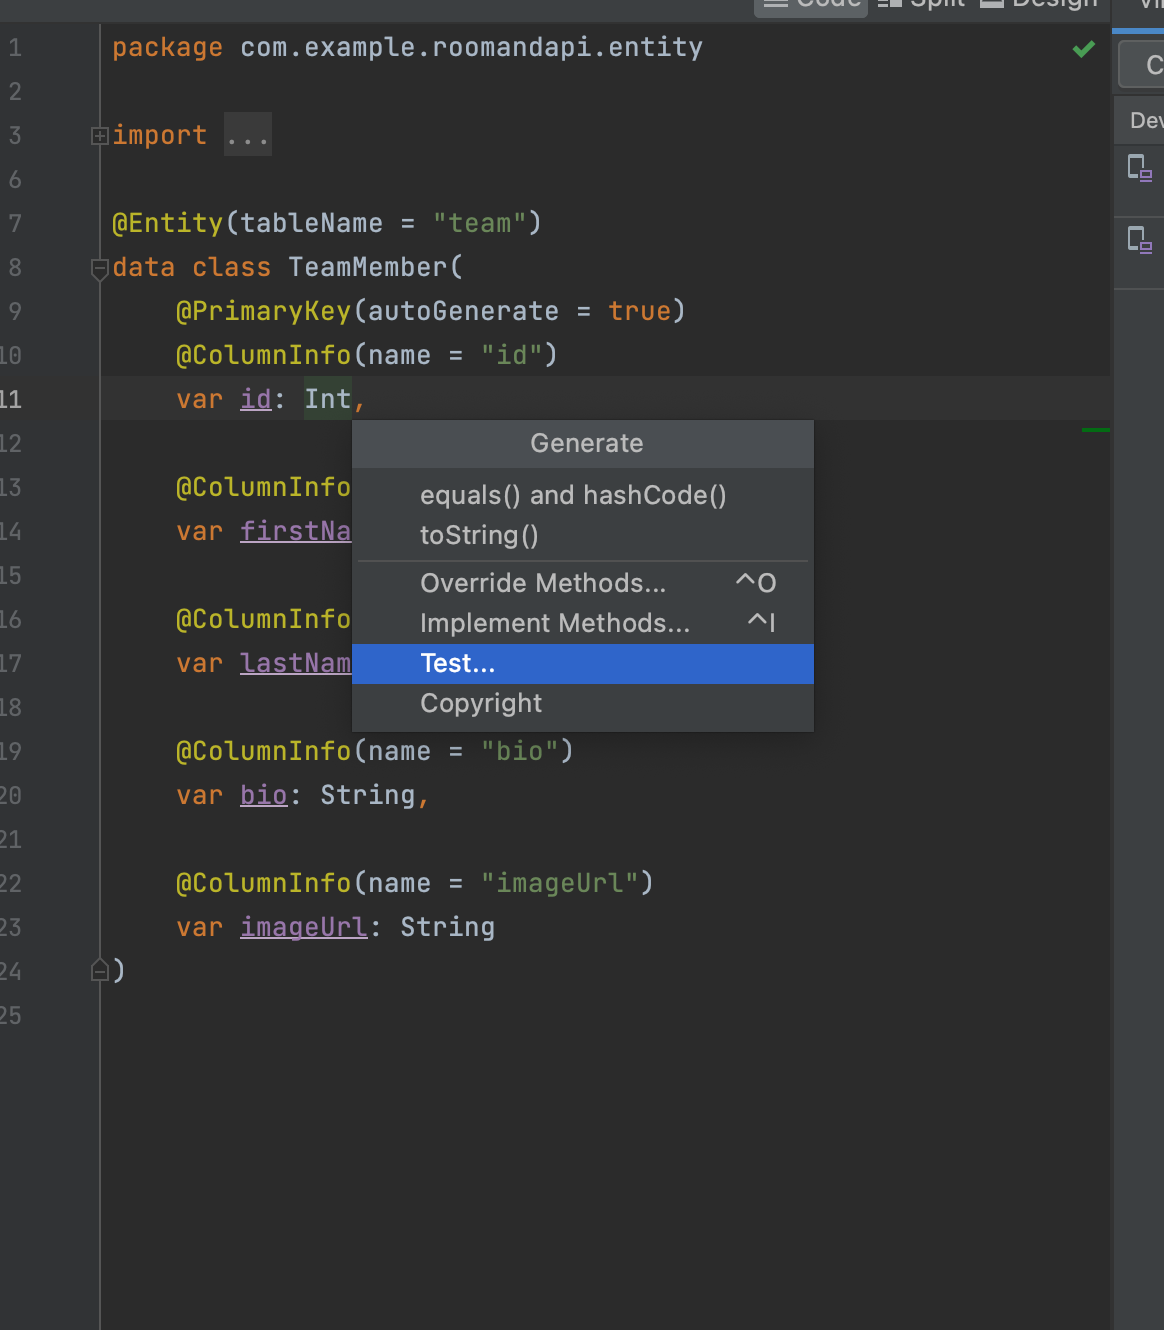
\includegraphics[trim=10 10 10 50, clip, width=\textwidth] {images/testing/2_generate_test.png}
    \caption{Step 2. Click Generate and then Click Test}
    \label{fig:test_step_2}
\end{figure}

From the \verb|Generate| menu, select \verb|Test...| to create a new test file as shown in Figure \ref{fig:test_step_2},

\begin{figure}[H]
    \centering
    % trim and clip are used to crop the image, trim=left bottom right top
    % width sets max width, height will be scaled appropriately
    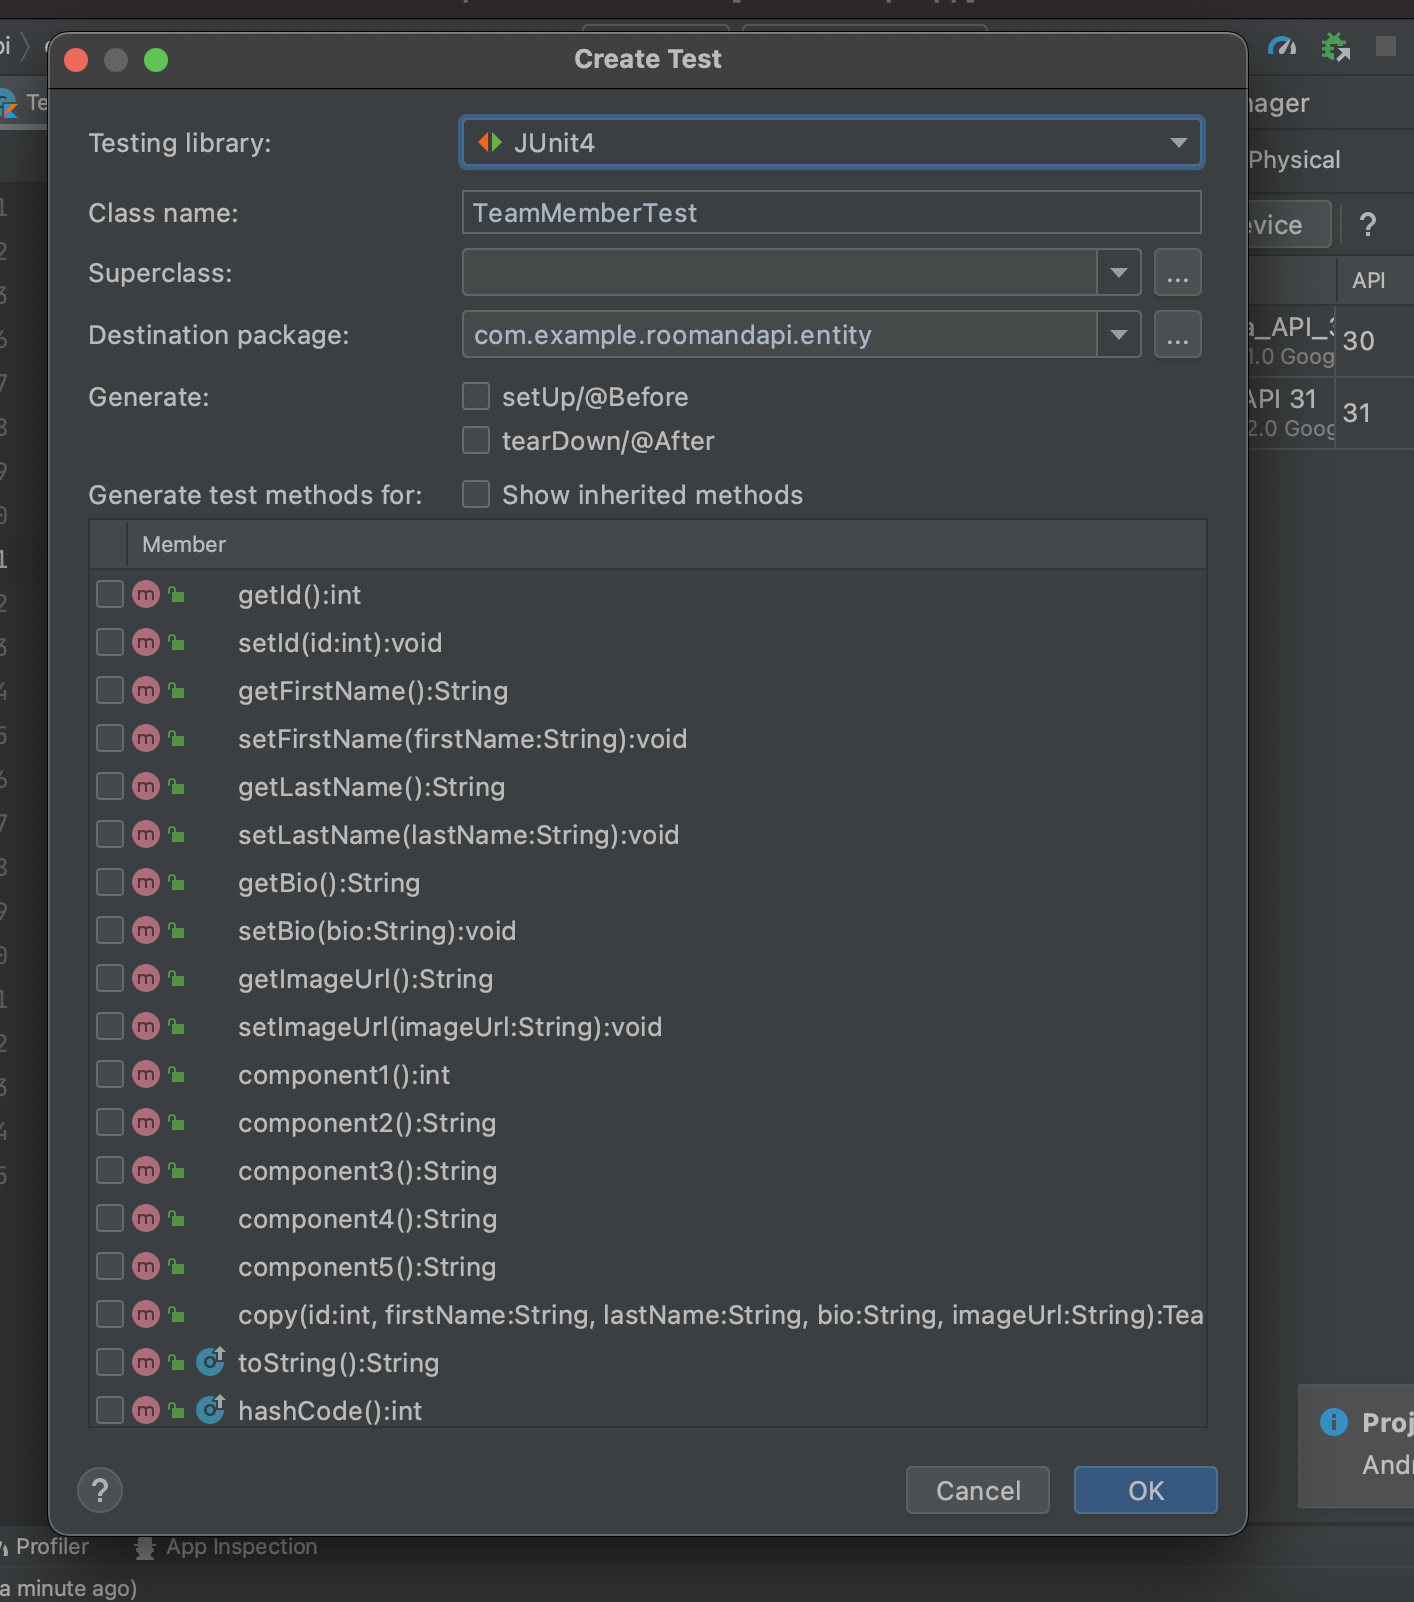
\includegraphics[trim=10 10 10 50, clip, width=\textwidth] {images/testing/3_pick_testing_Framework.png}
    \caption{Step 3, Select the version of JUnit to use}
    \label{fig:test_step_3}
\end{figure}
The \verb|Create Test| dialog box appears after selecting \verb|Test...|. In this dialog as shown in Figure \ref{fig:test_step_3}, the user can specify the type of testing framework to use with the \verb|Testing Library| dropdown. In this example, the JUnit4 testing library is used.

\begin{figure}[H]
    \centering
    % trim and clip are used to crop the image, trim=left bottom right top
    % width sets max width, height will be scaled appropriately
    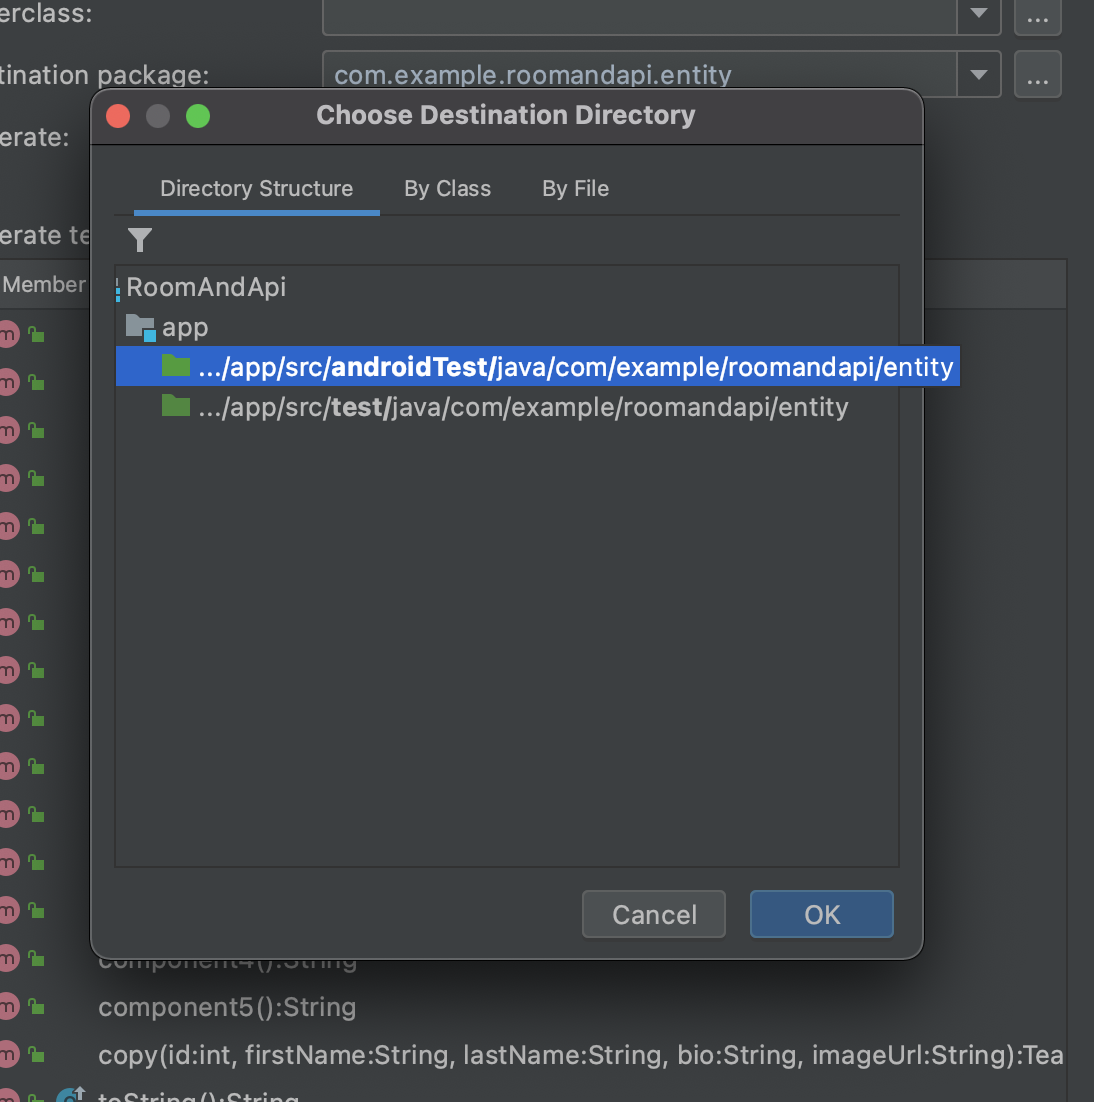
\includegraphics[trim=10 10 10 50, clip, width=\textwidth] {images/testing/4_pick_test_type.png}
    \caption{Step 4, Determine the type of test}
    \label{fig:test_step_4}
\end{figure}
 Then the \verb|OK| button can be clicked to move on to the \verb|Choose Destination| dialog box shown in Figure \ref{fig:test_step_4}. In this dialog box you can specify whether this will be an AndroidTest running within an emulator or a standard JUnit test by selecting the appropriate destination, AndroidTests or Tests. Since we are testing the RoomDatabase, the test has to be an Android Test and must stored in the AndroidTests directory

 \begin{figure}[H]
    \centering
    % trim and clip are used to crop the image, trim=left bottom right top
    % width sets max width, height will be scaled appropriately
    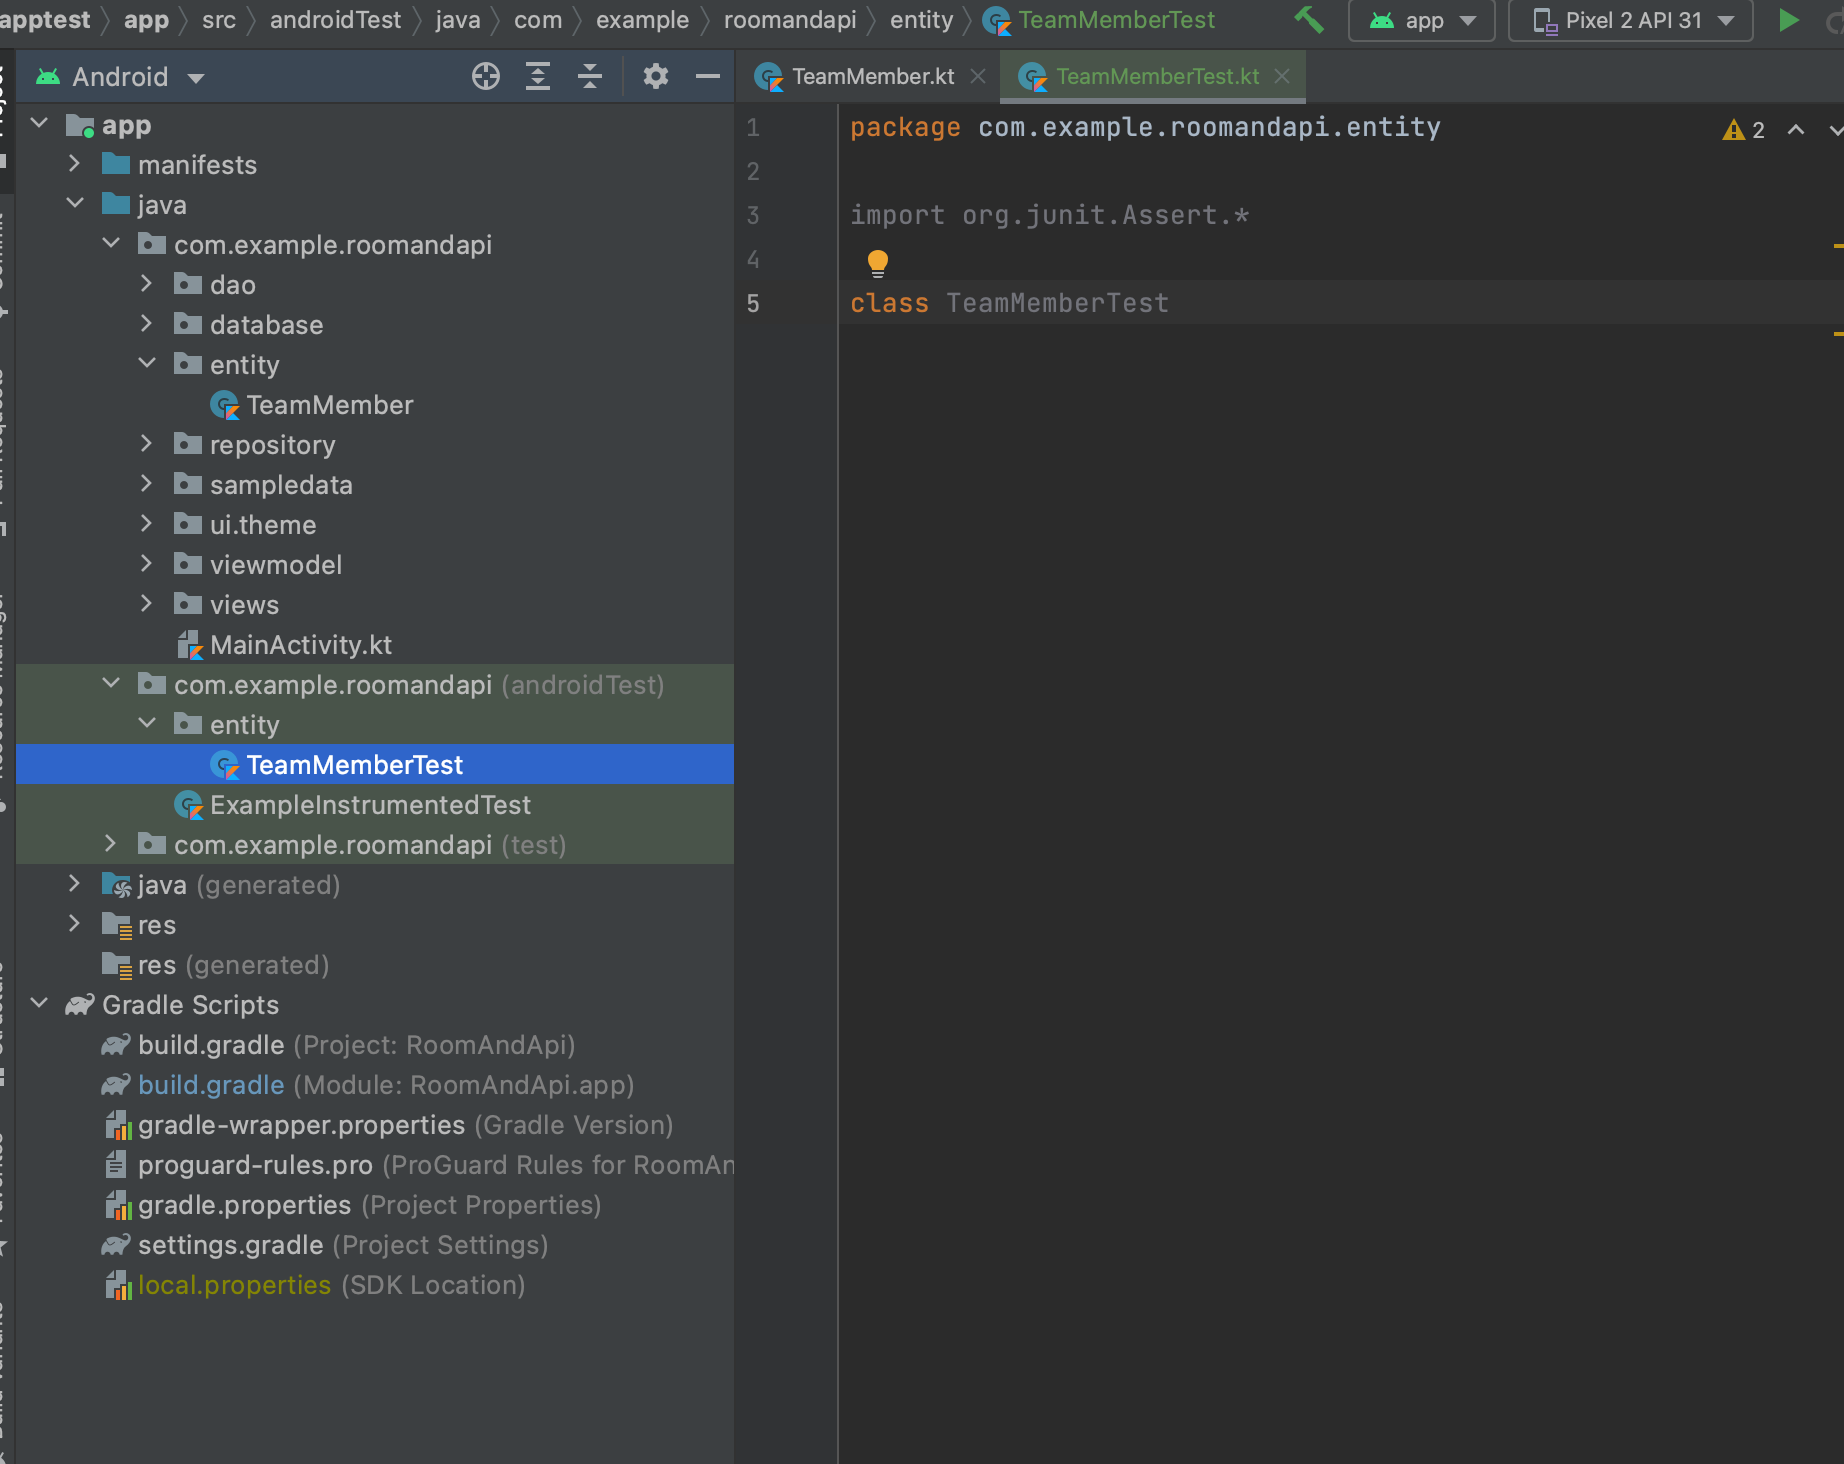
\includegraphics[trim=10 10 10 50, clip, width=\textwidth] {images/testing/5_result.png}
    \caption{Auto-generated Test Class}
    \label{fig:test_step_5}
\end{figure}
 
 After following those steps, a skeleton of an  Android Test class will be created . In order to get the class to run properly, an annotation \verb|@RunWith(AndroidJUnit4::class)| needs to be added at the front of the class. The class header will also need to extend the TestCase class using the heading \verb|class nameOfClass: TestCase(){| After that has been created, common variables need to be created as members of the class. When testing the Room Database, the private members should include an instance of the database, the dao being tested and possibly the repository if the repository is being tested.  

 \begin{lstlisting}[numbers=none, 
			caption=Code to Set up the Database in Test,
			label={lst:before_testing}]
@Before
    public override fun setUp(){
        val context = ApplicationProvider.getApplicationContext<Context>()
        db = Room.inMemoryDatabaseBuilder(context, WCDatabase::class.java).build()
        dao = db.userDao()
    }
\end{lstlisting}
 Since the database will have to be created with every test,  the \verb|@Before| annotation is needed to define the code to generate the database. Listing \ref{lst:before_testing} contains a \verb|setUp()| function which is used to create a an \verb|inMemoryDatabase| which is a database that is loaded into memory but does not persist after it is closed, which makes it ideal for testing. The inMemoryDatabase is created using Room's \verb|inMemoryDatabseBuilder| class which takes the application context and the class of the database to instantiate with the build() method. Once the database is created, the dao is instantiated from the appropriate database method.

   \begin{lstlisting}[numbers=none, 
			caption=Code to close the Database after the test,
			label={lst:after_testing}]
    @After
    fun closeDB(){
        db.close()
    }
\end{lstlisting}

Since every test is going to have to close the databse, the \verb|@After| annotation is used to create a function that is run after each test to close the database. An example of this function is shown in Listing \ref{lst:after_testing}. The function \verb|closeDB()| simply abstracts the database's close method and calls it. 

   \begin{lstlisting}[numbers=none, 
			caption=Example Test for Room Database,
			label={lst:example_room_test}]
    @Test
    fun TestWriteAndReadUser() = runBlocking(){
        val members: List<TeamMember> =  listOf(
            TeamMember(1,
            "Jacob",
            "Conner",
            "Jacob Conner is a senior at Old Dominion University majoring in Computer Science. Currently, he lives in Blacksburg, Virginia, and works in a chat-based technical support role for Dish Network. Some of his hobbies include archaeology, learning Japanese and browsing Linkedin Learning.",
            "https://www.cs.odu.edu/~cpi/old/410/silvers21/bio/Jacob_Conner.jpg")
        )
        dao.insert(members)
        val byName: TeamMember = dao.getByName("Jacob", "Conner")
        MatcherAssert.assertThat(byName, CoreMatchers.equalTo(members[0]))
    }
\end{lstlisting}

Now that the initial setup has been created, tests for the database can be created. A test is annotated with  \verb|@Test| before the test function.  Each function is set up with runBlocking to force the thread used to call the test to wait until the test finishes \cite{kotlinCoroutines}.  Then the test is setup with anything particular to the test. In Listing \ref{lst:example_room_test} the database's ability to insert and read data is tested by creating an instance of a team member. This team member is inserted into the database using the dao's insert method. The database is read to create a new instance of the team member which should be the same as the team member just inserted with the dao's getByName method. The MatcherAssert.assertThat method is used to test if the two TeamMember entities are equal. If they are equal, the test passes \cite{SimplifiedCodingRoomTesting}. 

\lstinputlisting[language=Java, caption=Example entity test class, label={lst:exampleEntityTest}]{app/src/androidTest/java/com/example/roomandapi/entity/TeamMemberTest.kt}

The example test file for the TeamMember class is shown in listing \ref{lst:exampleEntityTest}. 


\section{JetPack Compose}

\subsection{Navigation}
Navigation in JetPack Compose consists of a NavController to provide the routes to the various views and buttons on the view to navigate to those routes \cite{mediumJetpackNavigation} \cite{NavigationCodeLab}. 
\lstinputlisting[language=Java, caption=Example Activty View with a NavController, label={lst:exampleNavView}]{app/src/main/java/com/example/roomandapi/views/MainView.kt}


\begin{lstlisting}[numbers=none, 
			caption=Function to create a simple Nav Controller,
			label={lst:navControllerFunction}]
@Composable
fun appNavController() {

    val navController = rememberNavController()
    //default destination
    NavHost(navController, startDestination = "nameOfDefaultRoute") {
    	//list routes
        composable(route = "<nameOfFirstRoute>") {
        	    //viewToLoad
	    firstView(navController)
        }
        
        composable(route = "<nameOfSecondRoute>") {
	    secondView(navController)
        }
    }
}
\end{lstlisting}

In the navController function shown in listing \ref{lst:navControllerFunction}, the navController begins like all composable functions with the \verb|@Composable| annotation. Then the name of the function for the navController is defined. Since the nav controller manages routes, a state variable needs to be handled to keep track of the current route. This state is defined as navController in the example code and is created using the \verb|rememberNavController()| method. Next the NavHost is created which takes the state, and the default or \verb|startDestination|. Within the NavHost function, the \verb|composable| method is called for each route. This method simply takes the route which has a string for the name of the route. Inside of this function, the view that should be loaded with that particular route. Since we need to keep track of the current route, each view used in a navController should require the remembered navController..  
\begin{lstlisting}[numbers=none, 
			caption=Button to navigate to a view,
			label={lst:navButton}]
Button(onClick = { navController.navigate("<routeToNavigateTo") }) {
                //Label for button
                Text("Name of Button")
            }
}
\end{lstlisting}

In order to move between routes, a Button component can be created like the one shown in Listing \ref{lst:navButton}. To make the button switch to a different route, the \verb|onClick| argument needs to be set to \verb|navController.navigate("nameOfRoute")|. Then normal styling can be used inside of the button. For example, a label can be set with the Text component with the Text property set to the name of the button. The text property's \verb|text=| can be omitted when the text is the only property set \cite{mediumJetpackNavigation}.  

\subsection{Handling Remote Resources - Images}
\begin{lstlisting}[numbers=none, 
			caption=Coil Dependency,
			label={lst:coilDependency}]
implementation("io.coil-kt:coil-compose:1.3.1")
\end{lstlisting}
Some APIs may make use of Image files referred to remotely and there are instances when we would like the application to download an image from the web and use that image in the web. In order to support this, the \verb|Coil| library can be imported by adding the dependency in Listing \ref{lst:coilDependency} into the application's \textit{build.gradle} file. 

\begin{lstlisting}[numbers=none, 
			caption=Example Image using Coil,
			label={lst:exampleWithCoil}]
Image(
                        painter = rememberImagePainter("https://www.cs.odu.edu/~cpi/old/410/silvers21/bio/Jacob\_Conner.jpg"),
                        contentDescription = null,
                        modifier = Modifier.size(128.dp)
                    )
\end{lstlisting}


Once the dependency has been imported, the image urls can be loaded in the app by creating an \verb|Image| composable function and setting the painter property with the \verb|rememberImagePainter| function that takes the url as an argument \cite{StackOverflowCoil}. An example image composable to load a remote resource is shown in Listing \ref{lst:exampleWithCoil}.

                    

\section{Documenting with Dokka}
test
\begin{appendix}
  \listoffigures
  \newpage
  \listoftables
  \newpage
  \lstlistoflistings

\end{appendix}
\newpage
\RaggedRight
\bibliography{references}{}
 \bibliographystyle{elsarticle-num} 
\end{document}